\batchmode
\documentclass[twoside]{article}

% Packages required by doxygen
\usepackage{calc}
\usepackage{doxygen}
\usepackage{graphicx}
\usepackage[utf8]{inputenc}
\usepackage{makeidx}
\usepackage{multicol}
\usepackage{multirow}
\usepackage{textcomp}
\usepackage[table]{xcolor}

% Font selection
\usepackage[T1]{fontenc}
\usepackage{mathptmx}
\usepackage[scaled=.90]{helvet}
\usepackage{courier}
\usepackage{amssymb}
\usepackage{sectsty}
\renewcommand{\familydefault}{\sfdefault}
\allsectionsfont{%
  \fontseries{bc}\selectfont%
  \color{darkgray}%
}
\renewcommand{\DoxyLabelFont}{%
  \fontseries{bc}\selectfont%
  \color{darkgray}%
}

% Page & text layout
\usepackage{geometry}
\geometry{%
  letterpaper,%
  top=2.5cm,%
  bottom=2.5cm,%
  left=2.5cm,%
  right=2.5cm%
}
\tolerance=750
\hfuzz=15pt
\hbadness=750
\setlength{\emergencystretch}{15pt}
\setlength{\parindent}{0cm}
\setlength{\parskip}{0.2cm}
\makeatletter
\renewcommand{\paragraph}{%
  \@startsection{paragraph}{4}{0ex}{-1.0ex}{1.0ex}{%
    \normalfont\normalsize\bfseries\SS@parafont%
  }%
}
\renewcommand{\subparagraph}{%
  \@startsection{subparagraph}{5}{0ex}{-1.0ex}{1.0ex}{%
    \normalfont\normalsize\bfseries\SS@subparafont%
  }%
}
\makeatother

% Headers & footers
\usepackage{fancyhdr}
\pagestyle{fancyplain}
\fancyhead[LE]{\fancyplain{}{\bfseries\thepage}}
\fancyhead[CE]{\fancyplain{}{}}
\fancyhead[RE]{\fancyplain{}{\bfseries\leftmark}}
\fancyhead[LO]{\fancyplain{}{\bfseries\rightmark}}
\fancyhead[CO]{\fancyplain{}{}}
\fancyhead[RO]{\fancyplain{}{\bfseries\thepage}}
\fancyfoot[LE]{\fancyplain{}{}}
\fancyfoot[CE]{\fancyplain{}{}}
\fancyfoot[RE]{\fancyplain{}{\bfseries\scriptsize Generated on Sat Feb 16 2019 22\-:42\-:19 for Backtrace\-Exception by Doxygen }}
\fancyfoot[LO]{\fancyplain{}{\bfseries\scriptsize Generated on Sat Feb 16 2019 22\-:42\-:19 for Backtrace\-Exception by Doxygen }}
\fancyfoot[CO]{\fancyplain{}{}}
\fancyfoot[RO]{\fancyplain{}{}}
\renewcommand{\footrulewidth}{0.4pt}
\renewcommand{\sectionmark}[1]{%
  \markright{\thesection\ #1}%
}

% Indices & bibliography
\usepackage{natbib}
\usepackage[titles]{tocloft}
\setcounter{tocdepth}{3}
\setcounter{secnumdepth}{5}
\makeindex

% Hyperlinks (required, but should be loaded last)
\usepackage{ifpdf}
\ifpdf
  \usepackage[pdftex,pagebackref=true]{hyperref}
\else
  \usepackage[ps2pdf,pagebackref=true]{hyperref}
\fi
\hypersetup{%
  colorlinks=true,%
  linkcolor=blue,%
  citecolor=blue,%
  unicode%
}

% Custom commands
\newcommand{\clearemptydoublepage}{%
  \newpage{\pagestyle{empty}\cleardoublepage}%
}


%===== C O N T E N T S =====

\begin{document}

% Titlepage & ToC
\hypersetup{pageanchor=false}
\pagenumbering{roman}
\begin{titlepage}
\vspace*{7cm}
\begin{center}%
{\Large Backtrace\-Exception }\\
\vspace*{1cm}
{\large Generated by Doxygen 1.8.6}\\
\vspace*{0.5cm}
{\small Sat Feb 16 2019 22:42:19}\\
\end{center}
\end{titlepage}
\tableofcontents
\pagenumbering{arabic}
\hypersetup{pageanchor=true}

%--- Begin generated contents ---
\section{Main Page}
\label{index}\hypertarget{index}{}Backtrace\-Exception is a C++ exception type that produces a backtrace when thrown. It can capture this backtrace with several methods and the backtrace can be disabled. The goal is for the library to work on both Linux and windows 64-\/bit.

\subsubsection*{Using Backtrace Exception}

\paragraph*{C\-Make configuration options}

\subsubsection*{Backtrace Methods}
\section{Namespace Index}
\subsection{Namespace List}
Here is a list of all namespaces with brief descriptions\-:\begin{DoxyCompactList}
\item\contentsline{section}{\hyperlink{namespacebacktrace__exception}{backtrace\-\_\-exception} }{\pageref{namespacebacktrace__exception}}{}
\end{DoxyCompactList}

\section{File Index}
\subsection{File List}
Here is a list of all files with brief descriptions\-:\begin{DoxyCompactList}
\item\contentsline{section}{\hyperlink{BacktraceException_8cpp}{Backtrace\-Exception.\-cpp} \\*Backtrace\-Exception class member function definitions }{\pageref{BacktraceException_8cpp}}{}
\item\contentsline{section}{\hyperlink{BacktraceException_8h}{Backtrace\-Exception.\-h} \\*Backtrace\-Exception class declaration and inline member functions }{\pageref{BacktraceException_8h}}{}
\end{DoxyCompactList}

\section{Namespace Documentation}
\hypertarget{namespacebacktrace__exception}{}\subsection{backtrace\+\_\+exception Namespace Reference}
\label{namespacebacktrace__exception}\index{backtrace\+\_\+exception@{backtrace\+\_\+exception}}
\subsubsection*{Classes}
\begin{DoxyCompactItemize}
\item 
class \hyperlink{classbacktrace__exception_1_1BacktraceException}{Backtrace\+Exception}
\begin{DoxyCompactList}\small\item\em Extension of std\+::exception that produces saved backtraces for debugging. \end{DoxyCompactList}\end{DoxyCompactItemize}
\subsubsection*{Enumerations}
\begin{DoxyCompactItemize}
\item 
enum \hyperlink{namespacebacktrace__exception_ac04b358e6d3eac08b792a7c2e99b57cc}{Backtrace\+Method} \{ \hyperlink{namespacebacktrace__exception_ac04b358e6d3eac08b792a7c2e99b57cca0ded6244fb02e7fb8db8e873d25656c5}{Backtrace\+Method\+::glibc}, 
\hyperlink{namespacebacktrace__exception_ac04b358e6d3eac08b792a7c2e99b57ccaca3e1c20efd5690f9789a87c66a5047a}{Backtrace\+Method\+::gdb}, 
\hyperlink{namespacebacktrace__exception_ac04b358e6d3eac08b792a7c2e99b57ccac87739aef758816341a559291c49bbbb}{Backtrace\+Method\+::stackwalk}
 \}
\end{DoxyCompactItemize}
\subsubsection*{Functions}
\begin{DoxyCompactItemize}
\item 
\hyperlink{namespacebacktrace__exception_ac04b358e6d3eac08b792a7c2e99b57cc}{Backtrace\+Method} \hyperlink{namespacebacktrace__exception_a024cd6e7707e7f7cbb9283e60907142c}{get\+\_\+backtrace\+\_\+method} ()
\item 
void \hyperlink{namespacebacktrace__exception_afe7dd97c0deefd1a0e9cb08f9c8089b2}{set\+\_\+backtrace\+\_\+method} (\hyperlink{namespacebacktrace__exception_ac04b358e6d3eac08b792a7c2e99b57cc}{Backtrace\+Method} method)
\item 
void \hyperlink{namespacebacktrace__exception_a134895cbad5bc441a941f1f49b43a78a}{disable\+\_\+backtraces} ()
\item 
void \hyperlink{namespacebacktrace__exception_a4e1b86dea1b116c7bac88d89448a808e}{enable\+\_\+backtraces} ()
\item 
bool \hyperlink{namespacebacktrace__exception_a68f7b8565eefc4f9b862c25ec47ce2b7}{backtraces\+\_\+enabled} ()
\end{DoxyCompactItemize}


\subsubsection{Enumeration Type Documentation}
\index{backtrace\+\_\+exception@{backtrace\+\_\+exception}!Backtrace\+Method@{Backtrace\+Method}}
\index{Backtrace\+Method@{Backtrace\+Method}!backtrace\+\_\+exception@{backtrace\+\_\+exception}}
\paragraph[{\texorpdfstring{Backtrace\+Method}{BacktraceMethod}}]{\setlength{\rightskip}{0pt plus 5cm}enum {\bf backtrace\+\_\+exception\+::\+Backtrace\+Method}\hspace{0.3cm}{\ttfamily [strong]}}\hypertarget{namespacebacktrace__exception_ac04b358e6d3eac08b792a7c2e99b57cc}{}\label{namespacebacktrace__exception_ac04b358e6d3eac08b792a7c2e99b57cc}
\begin{Desc}
\item[Enumerator]\par
\begin{description}
\index{glibc@{glibc}!backtrace\+\_\+exception@{backtrace\+\_\+exception}}\index{backtrace\+\_\+exception@{backtrace\+\_\+exception}!glibc@{glibc}}\item[{\em 
glibc\hypertarget{namespacebacktrace__exception_ac04b358e6d3eac08b792a7c2e99b57cca0ded6244fb02e7fb8db8e873d25656c5}{}\label{namespacebacktrace__exception_ac04b358e6d3eac08b792a7c2e99b57cca0ded6244fb02e7fb8db8e873d25656c5}
}]\index{gdb@{gdb}!backtrace\+\_\+exception@{backtrace\+\_\+exception}}\index{backtrace\+\_\+exception@{backtrace\+\_\+exception}!gdb@{gdb}}\item[{\em 
gdb\hypertarget{namespacebacktrace__exception_ac04b358e6d3eac08b792a7c2e99b57ccaca3e1c20efd5690f9789a87c66a5047a}{}\label{namespacebacktrace__exception_ac04b358e6d3eac08b792a7c2e99b57ccaca3e1c20efd5690f9789a87c66a5047a}
}]\index{stackwalk@{stackwalk}!backtrace\+\_\+exception@{backtrace\+\_\+exception}}\index{backtrace\+\_\+exception@{backtrace\+\_\+exception}!stackwalk@{stackwalk}}\item[{\em 
stackwalk\hypertarget{namespacebacktrace__exception_ac04b358e6d3eac08b792a7c2e99b57ccac87739aef758816341a559291c49bbbb}{}\label{namespacebacktrace__exception_ac04b358e6d3eac08b792a7c2e99b57ccac87739aef758816341a559291c49bbbb}
}]\end{description}
\end{Desc}


Definition at line 16 of file Backtrace\+Exception.\+h.



\subsubsection{Function Documentation}
\index{backtrace\+\_\+exception@{backtrace\+\_\+exception}!backtraces\+\_\+enabled@{backtraces\+\_\+enabled}}
\index{backtraces\+\_\+enabled@{backtraces\+\_\+enabled}!backtrace\+\_\+exception@{backtrace\+\_\+exception}}
\paragraph[{\texorpdfstring{backtraces\+\_\+enabled()}{backtraces_enabled()}}]{\setlength{\rightskip}{0pt plus 5cm}bool backtrace\+\_\+exception\+::backtraces\+\_\+enabled (
\begin{DoxyParamCaption}
{}
\end{DoxyParamCaption}
)}\hypertarget{namespacebacktrace__exception_a68f7b8565eefc4f9b862c25ec47ce2b7}{}\label{namespacebacktrace__exception_a68f7b8565eefc4f9b862c25ec47ce2b7}


Definition at line 84 of file Backtrace\+Exception.\+cpp.



Referenced by backtrace\+\_\+exception\+::\+Backtrace\+Exception\+::print\+\_\+backtrace(), and backtrace\+\_\+exception\+::\+Backtrace\+Exception\+::what().



Here is the caller graph for this function\+:\nopagebreak
\begin{figure}[H]
\begin{center}
\leavevmode
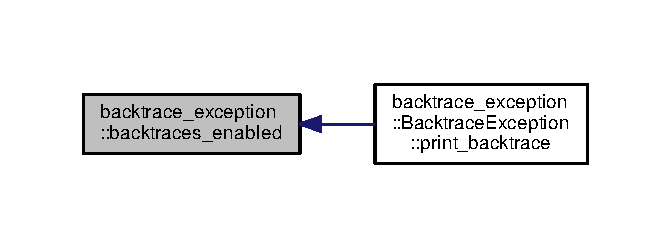
\includegraphics[width=346pt]{namespacebacktrace__exception_a68f7b8565eefc4f9b862c25ec47ce2b7_icgraph}
\end{center}
\end{figure}


\index{backtrace\+\_\+exception@{backtrace\+\_\+exception}!disable\+\_\+backtraces@{disable\+\_\+backtraces}}
\index{disable\+\_\+backtraces@{disable\+\_\+backtraces}!backtrace\+\_\+exception@{backtrace\+\_\+exception}}
\paragraph[{\texorpdfstring{disable\+\_\+backtraces()}{disable_backtraces()}}]{\setlength{\rightskip}{0pt plus 5cm}void backtrace\+\_\+exception\+::disable\+\_\+backtraces (
\begin{DoxyParamCaption}
{}
\end{DoxyParamCaption}
)}\hypertarget{namespacebacktrace__exception_a134895cbad5bc441a941f1f49b43a78a}{}\label{namespacebacktrace__exception_a134895cbad5bc441a941f1f49b43a78a}


Definition at line 74 of file Backtrace\+Exception.\+cpp.

\index{backtrace\+\_\+exception@{backtrace\+\_\+exception}!enable\+\_\+backtraces@{enable\+\_\+backtraces}}
\index{enable\+\_\+backtraces@{enable\+\_\+backtraces}!backtrace\+\_\+exception@{backtrace\+\_\+exception}}
\paragraph[{\texorpdfstring{enable\+\_\+backtraces()}{enable_backtraces()}}]{\setlength{\rightskip}{0pt plus 5cm}void backtrace\+\_\+exception\+::enable\+\_\+backtraces (
\begin{DoxyParamCaption}
{}
\end{DoxyParamCaption}
)}\hypertarget{namespacebacktrace__exception_a4e1b86dea1b116c7bac88d89448a808e}{}\label{namespacebacktrace__exception_a4e1b86dea1b116c7bac88d89448a808e}


Definition at line 79 of file Backtrace\+Exception.\+cpp.

\index{backtrace\+\_\+exception@{backtrace\+\_\+exception}!get\+\_\+backtrace\+\_\+method@{get\+\_\+backtrace\+\_\+method}}
\index{get\+\_\+backtrace\+\_\+method@{get\+\_\+backtrace\+\_\+method}!backtrace\+\_\+exception@{backtrace\+\_\+exception}}
\paragraph[{\texorpdfstring{get\+\_\+backtrace\+\_\+method()}{get_backtrace_method()}}]{\setlength{\rightskip}{0pt plus 5cm}{\bf Backtrace\+Method} backtrace\+\_\+exception\+::get\+\_\+backtrace\+\_\+method (
\begin{DoxyParamCaption}
{}
\end{DoxyParamCaption}
)}\hypertarget{namespacebacktrace__exception_a024cd6e7707e7f7cbb9283e60907142c}{}\label{namespacebacktrace__exception_a024cd6e7707e7f7cbb9283e60907142c}


Definition at line 46 of file Backtrace\+Exception.\+cpp.

\index{backtrace\+\_\+exception@{backtrace\+\_\+exception}!set\+\_\+backtrace\+\_\+method@{set\+\_\+backtrace\+\_\+method}}
\index{set\+\_\+backtrace\+\_\+method@{set\+\_\+backtrace\+\_\+method}!backtrace\+\_\+exception@{backtrace\+\_\+exception}}
\paragraph[{\texorpdfstring{set\+\_\+backtrace\+\_\+method(\+Backtrace\+Method method)}{set_backtrace_method(BacktraceMethod method)}}]{\setlength{\rightskip}{0pt plus 5cm}void backtrace\+\_\+exception\+::set\+\_\+backtrace\+\_\+method (
\begin{DoxyParamCaption}
\item[{{\bf Backtrace\+Method}}]{method}
\end{DoxyParamCaption}
)}\hypertarget{namespacebacktrace__exception_afe7dd97c0deefd1a0e9cb08f9c8089b2}{}\label{namespacebacktrace__exception_afe7dd97c0deefd1a0e9cb08f9c8089b2}


Definition at line 51 of file Backtrace\+Exception.\+cpp.



References gdb, glibc, and stackwalk.


\section{File Documentation}
\hypertarget{BacktraceException_8cpp}{\subsection{Backtrace\-Exception.\-cpp File Reference}
\label{BacktraceException_8cpp}\index{Backtrace\-Exception.\-cpp@{Backtrace\-Exception.\-cpp}}
}


Backtrace\-Exception class member function definitions.  


{\ttfamily \#include \char`\"{}Backtrace\-Exception/\-Backtrace\-Exception.\-h\char`\"{}}\\*
{\ttfamily \#include $<$cstdlib$>$}\\*
{\ttfamily \#include $<$memory$>$}\\*
{\ttfamily \#include $<$iostream$>$}\\*
{\ttfamily \#include $<$string$>$}\\*
{\ttfamily \#include $<$sstream$>$}\\*
{\ttfamily \#include $<$vector$>$}\\*
Include dependency graph for Backtrace\-Exception.\-cpp\-:\nopagebreak
\begin{figure}[H]
\begin{center}
\leavevmode
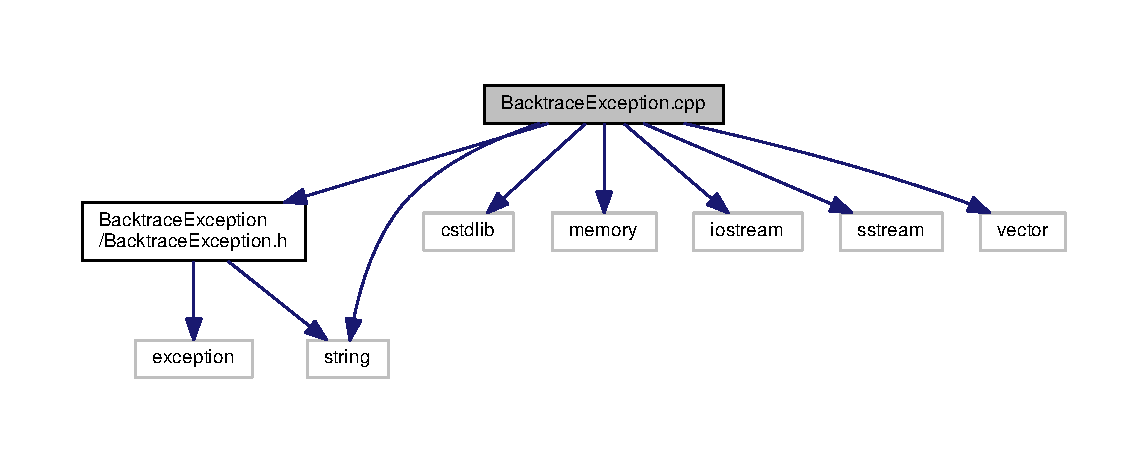
\includegraphics[width=350pt]{BacktraceException_8cpp__incl}
\end{center}
\end{figure}
\subsubsection*{Namespaces}
\begin{DoxyCompactItemize}
\item 
\hyperlink{namespacebacktrace__exception}{backtrace\-\_\-exception}
\end{DoxyCompactItemize}
\subsubsection*{Functions}
\begin{DoxyCompactItemize}
\item 
Backtrace\-Method \hyperlink{namespacebacktrace__exception_a024cd6e7707e7f7cbb9283e60907142c}{backtrace\-\_\-exception\-::get\-\_\-backtrace\-\_\-method} ()
\item 
void \hyperlink{namespacebacktrace__exception_afe7dd97c0deefd1a0e9cb08f9c8089b2}{backtrace\-\_\-exception\-::set\-\_\-backtrace\-\_\-method} (Backtrace\-Method method)
\item 
void \hyperlink{namespacebacktrace__exception_a134895cbad5bc441a941f1f49b43a78a}{backtrace\-\_\-exception\-::disable\-\_\-backtraces} ()
\item 
void \hyperlink{namespacebacktrace__exception_a4e1b86dea1b116c7bac88d89448a808e}{backtrace\-\_\-exception\-::enable\-\_\-backtraces} ()
\item 
bool \hyperlink{namespacebacktrace__exception_a68f7b8565eefc4f9b862c25ec47ce2b7}{backtrace\-\_\-exception\-::backtraces\-\_\-enabled} ()
\end{DoxyCompactItemize}


\subsubsection{Detailed Description}
Backtrace\-Exception class member function definitions. \begin{DoxyAuthor}{Author}
Mark J. Olah (mjo@cs.\-unm D\-O\-T edu) 
\end{DoxyAuthor}
\begin{DoxyDate}{Date}
2017 -\/ 2018 
\end{DoxyDate}
\begin{DoxyCopyright}{Copyright}
Licensed under the Apache License, Version 2.\-0. See L\-I\-C\-E\-N\-S\-E file. 
\end{DoxyCopyright}


Definition in file \hyperlink{BacktraceException_8cpp_source}{Backtrace\-Exception.\-cpp}.


\hypertarget{README_8md}{\subsection{R\-E\-A\-D\-M\-E.\-md File Reference}
\label{README_8md}\index{R\-E\-A\-D\-M\-E.\-md@{R\-E\-A\-D\-M\-E.\-md}}
}

%--- End generated contents ---

% Index
\newpage
\phantomsection
\addcontentsline{toc}{section}{Index}
\printindex

\end{document}
